\RequirePackage[T1]{fontenc}
\documentclass[10pt,conference]{IEEEtran}
\IEEEoverridecommandlockouts
\usepackage{cite}
\usepackage{amsmath,amssymb}
\usepackage{graphicx}
\usepackage{booktabs}
\usepackage{multirow}
\usepackage{xcolor}
\usepackage{url}
\usepackage[hidelinks]{hyperref}
\usepackage{balance}

% Effective archived numeric values; later historical renewals consolidated.
\newcommand{\pctResolvedLite}{32.0}
\newcommand{\nResolvedLite}{96}
\newcommand{\nTotalLite}{300}
\newcommand{\strictRAPLite}{6.25}
\newcommand{\strictFalseRejLite}{94.79}
\newcommand{\strictGapLite}{30.0}
\newcommand{\strictMcNemarLite}{1.0}
\newcommand{\calRAPLite}{70.83}
\newcommand{\calRAPloLite}{61.08}
\newcommand{\calRAPhiLite}{78.98}
\newcommand{\calMRRLite}{22.67}
\newcommand{\calGapLite}{9.33}
\newcommand{\calGoldMergeLite}{72.92}
\newcommand{\calFalseRejLite}{27.08}
\newcommand{\calMcNemarLite}{0.8238}
\newcommand{\calHallucLite}{3.12}
\newcommand{\strictSevenFalseRejLite}{30.21}
\newcommand{\calSevenFalseRejLite}{12.5}
\newcommand{\calSevenMcNemarLite}{1.0}
\newcommand{\calSevenRAPLite}{86.46}
\newcommand{\strictFourteenFalseRejLite}{94.79}
\newcommand{\calFourteenFalseRejLite}{27.08}
\newcommand{\calFourteenMcNemarLite}{0.8238}
\newcommand{\calFourteenRAPLite}{70.83}
\newcommand{\strictThirtyTwoFalseRejLite}{100.0}
\newcommand{\calThirtyTwoFalseRejLite}{43.75}
\newcommand{\calThirtyTwoMcNemarLite}{0.42436}
\newcommand{\calThirtyTwoRAPLite}{51.04}
\newcommand{\pctResolvedVerified}{38.8}
\newcommand{\nResolvedVerified}{194}
\newcommand{\nTotalVerified}{500}
\newcommand{\strictRAPVerified}{6.19}
\newcommand{\strictFalseRejVerified}{93.3}
\newcommand{\strictGapVerified}{36.4}
\newcommand{\strictMcNemarVerified}{1.0}
\newcommand{\calRAPVerified}{72.16}
\newcommand{\calRAPloVerified}{65.47}
\newcommand{\calRAPhiVerified}{77.99}
\newcommand{\calMRRVerified}{28.0}
\newcommand{\calGapVerified}{10.8}
\newcommand{\calGoldMergeVerified}{74.74}
\newcommand{\calFalseRejVerified}{25.26}
\newcommand{\calMcNemarVerified}{0.49956}
\newcommand{\calHallucVerified}{4.64}
\newcommand{\strictSevenFalseRejVerified}{29.38}
\newcommand{\calSevenFalseRejVerified}{12.89}
\newcommand{\calSevenMcNemarVerified}{0.15159}
\newcommand{\calSevenRAPVerified}{91.24}
\newcommand{\strictFourteenFalseRejVerified}{93.3}
\newcommand{\calFourteenFalseRejVerified}{25.26}
\newcommand{\calFourteenMcNemarVerified}{0.49956}
\newcommand{\calFourteenRAPVerified}{72.16}
\newcommand{\strictThirtyTwoFalseRejVerified}{99.48}
\newcommand{\calThirtyTwoFalseRejVerified}{38.14}
\newcommand{\calThirtyTwoMcNemarVerified}{0.34968}
\newcommand{\calThirtyTwoRAPVerified}{57.73}
\newcommand{\fleissAllLite}{0.1008}
\newcommand{\fleissAgentLite}{0.1327}
\newcommand{\fleissAllVerified}{0.1172}
\newcommand{\fleissAgentVerified}{0.1222}
\newcommand{\dilemmaR}{0.994}
\newcommand{\dilemmaGap}{3.5}
\newcommand{\frontGold}{98.5}
\newcommand{\frontAgent}{84.5}
\newcommand{\frontFalseRej}{1.5}
\newcommand{\frontMcNemar}{<0.001}
\newcommand{\frontNvalid}{388}
\newcommand{\frontNpair}{194}
\newcommand{\frontAgentN}{194}
\newcommand{\frontGoldN}{194}
\newcommand{\frontKappaHuman}{0.167}
\newcommand{\frontGapPt}{13.9}
\newcommand{\frontGapCIlo}{8.8}
\newcommand{\frontGapCIhi}{19.6}
\newcommand{\frontKappaHumanFull}{0.167}
\newcommand{\negFailSeven}{84.1}
\newcommand{\negGoldSeven}{87.1}
\newcommand{\negGapSeven}{3.0}
\newcommand{\negFailFourteen}{66.2}
\newcommand{\negGoldFourteen}{74.7}
\newcommand{\negGapFourteen}{8.5}
\newcommand{\negN}{302}
\newcommand{\negFailThirtyTwo}{39.7}
\newcommand{\negGoldThirtyTwo}{61.9}
\newcommand{\negFailLlama}{86.1}
\newcommand{\negGoldLlama}{82.5}
\newcommand{\negFailDscoder}{44.9}
\newcommand{\negGoldDscoder}{38.0}
\newcommand{\negDscoderN}{296}
\newcommand{\negFailFrontier}{53.1}
\newcommand{\negGapFrontier}{45.4}
\newcommand{\negFrontierN}{81}
\newcommand{\negFailFrontierLo}{42.3}
\newcommand{\negFailFrontierHi}{63.6}


\setlength{\tabcolsep}{4pt}

\begin{document}

\title{Beyond \%Resolved:Reassessing SWE-bench Through Human and LLM Code Review}


\author{\IEEEauthorblockN{Myeongmuk Kang and Geunseok Yang\thanks{Corresponding author: Geunseok Yang (gsyang@hknu.ac.kr).}}
\IEEEauthorblockA{Department of Computer Science and Engineering, Hankyong National University\\
Anseong, Republic of Korea\\
Email: \{myoungmuk819, gsyang\}@hknu.ac.kr\\
ORCID: \href{https://orcid.org/0009-0002-5351-0269}{0009-0002-5351-0269} (Kang); \href{https://orcid.org/0000-0001-5677-5129}{0000-0001-5677-5129} (Yang)}}
\hypersetup{pdftitle={Beyond \%Resolved:Reassessing SWE-bench Through Human and LLM Code Review},
pdfauthor={Myeongmuk Kang and Geunseok Yang}}

\maketitle


\begin{abstract}
Passing benchmark tests does not establish that a maintainer would merge a coding-agent
patch. Large language model (LLM) reviewers offer a scalable additional assessment, but their
decisions also require validation. We study test-passing patches from four coding-agent
scaffolds on SWE-bench Lite and Verified, pairing agent patches with developer-merged gold
patches under source-blinded review. The headline naive reviewer, Qwen2.5-Coder-14B-AWQ,
rejects \strictFalseRejLite\% and \strictFalseRejVerified\% of the gold patches on Lite and
Verified. After jointly adjusting test-context disclosure and the merge-blocking rubric,
its gold rejection falls to \calFalseRejLite\% and \calFalseRejVerified\%; the same data were
used during rubric development and evaluation, so this is not independent calibration
validation. Across ten open-weight reviewer/prompt configurations on Verified, agent and
gold acceptance rates correlate at $r=0.994$, while agreement across five adjusted
reviewers is low (Fleiss $\kappa\approx0.02$). A hosted Claude reviewer accepts $164/194$
agent patches and $191/194$ paired gold patches (exact McNemar $p<0.001$), but its exact
model snapshot was not recorded and these decisions were not validated against maintainers.
The archived failing-patch comparison also supplied an incorrect test-pass assertion and
used different tasks; it cannot establish discrimination under correct test information.
A single non-independent rater's $40$-packet pilot provides descriptive observations only.
Our contribution is a control-based diagnosis of reviewer-dependent acceptance, together
with packets, verdicts, and analysis procedures. Historical gold acceptance is a useful
reference, but neither agreement with that reference nor a reviewer-specific agent--gold
difference establishes real-world mergeability.
\end{abstract}

\section{Introduction}
The dominant way to evaluate large language model (LLM) coding agents is execution-based:
SWE-bench~\cite{swebench} frames the task as ``GitHub issue $\rightarrow$ patch'' and
declares a task \emph{resolved} when the generated patch makes a held-out
\texttt{FAIL\_TO\_PASS} test pass while preserving \texttt{PASS\_TO\_PASS} tests. The
leaderboard metric \%Resolved has become the field's primary yardstick.

As execution scores rise, review-based criteria increasingly inform comparisons of coding
agents. LLMs make such assessments scalable, but interpreting a review score requires
checking the reviewer as well as the candidate.

Yet in real software development, passing tests is necessary but not sufficient for a change
to be accepted: a pull request must also survive \emph{code review}, where maintainers weigh
functional completeness, regression risk, minimality, maintainability, project conventions,
and test adequacy before merging~\cite{modernreview,tufanoreview}. That test-passing patches
can still be wrong is a long-standing observation in automated program repair, where
``plausible but incorrect'' patches and test overfitting have been studied for a
decade~\cite{overfitting,qirandom,patchcorrectness,patchsim}. For agentic software
engineering the concern is broader: the question is not only whether a multi-file,
agent-generated patch is \emph{correct} but whether it is \emph{mergeable}.

A natural research program follows: complement \%Resolved with a review-based criterion and
quantify the gap between them. Because human review at benchmark scale is expensive, the
obvious instrument is an LLM reviewer, mirroring the now-common LLM-as-judge
paradigm~\cite{llmjudge}. This paper asks whether that instrument actually works.


We operationalize review-based evaluation on test-passing Agentless~\cite{agentless}
patches from SWE-bench Lite and Verified~\cite{swebench,swebenchverified}. Each agent patch
and its developer-merged gold counterpart is rendered as a source-blinded review packet.
Gold acceptance measures agreement with a known historical merge outcome under those
packet conditions. It does not establish that a gold patch is defect-free or that a new
reviewer's objection is false. Our measured outcome is \emph{reviewer-specific acceptance},
which we distinguish from an original maintainer's merge decision throughout the paper.

For Qwen2.5-Coder-14B-AWQ, the naive prompt rejects
\strictFalseRejLite\%/\strictFalseRejVerified\% of gold patches on Lite/Verified.
Jointly adjusting test-context disclosure and the blocking criterion increases both agent
and gold acceptance. Because the changes were not ablated and development inspected the
same gold cohort, we report a configuration comparison and subgroup stability, not
independent calibration generalization or an identified cause.

The open reviewers show an empirical \emph{validity--discrimination tension}: configurations
with high historical-gold agreement can also accept most agent patches, while more rejecting
configurations can disagree with historical gold acceptance. Across five models and two
prompts, aggregate agent and gold acceptance correlate at $r=0.994$. This correlation does
not identify a per-patch decision mechanism. A hosted Claude reviewer provides a different
operating point: \frontAgent\% agent acceptance versus \frontGold\% gold acceptance on
\frontNpair{} paired tasks ($p\frontMcNemar$). That difference is specific to the archived
reviewer and rubric; the exact hosted model ID was not logged, and maintainer agreement
remains unvalidated. Moreover, the failing-patch comparison reused a false test-pass
assertion, so it supplies no clean confirmation of functional discrimination.

We examine reviewer scale within Qwen2.5-Coder, extend the comparison to Llama and DeepSeek,
and compare three adjusted Qwen reviewers on four coding-agent scaffolds. Reviewer choice
matters: low inter-reviewer agreement persists, and Qwen-32B detects agent--gold differences
for SWE-agent and OpenHands that Qwen-14B does not. A single non-independent human rater
adds a limited descriptive comparison, not a population-level human validation.

\noindent Our contributions are:
\begin{itemize}
\item A paired historical-gold comparison showing how reported review acceptance changes
with the reviewer and prompt, including the contrast between the naive and adjusted Qwen
configurations (\S\ref{sec:results}).
\item A documented diagnosis of limitations in control-based validation: reused calibration
tasks, joint prompt changes, different positive/negative task populations, and an incorrect
pass assertion in the archived negative-control condition (\S\ref{sec:design}).
\item Cross-model and cross-agent results that separate aggregate acceptance, paired
differences, and inter-reviewer agreement; these outcomes are not substitutes for
maintainer-level validation (\S\ref{sec:results}).
\item A replication package containing source-blinded packets, normalized verdicts, exact
prompts and schemas, analysis code, and the $40$-packet exploratory human pilot.
\end{itemize}
Control examples and human-guided rubrics have precedents~\cite{cihanreview,hitlpatch}.
Our contribution is the SWE-bench-specific historical-acceptance comparison and its
empirical diagnosis, not the first use of calibration or positive controls.

\section{Background}
\textbf{Execution-based agent evaluation.} SWE-bench~\cite{swebench} casts coding-agent
evaluation as resolving real GitHub issues and scores an attempt by running the repository's
test suite: a task is \emph{resolved} when the agent's patch turns the \texttt{FAIL\_TO\_PASS}
tests green without breaking the \texttt{PASS\_TO\_PASS} tests. SWE-bench Verified is a
500-task subset that human annotators confirmed to be well-specified and
solvable~\cite{swebenchverified}, partly in response to concerns that some original tasks were
under-specified or had weak tests. A large ecosystem of scaffolds (Agentless~\cite{agentless},
SWE-agent~\cite{sweagent}, OpenHands~\cite{wang2024openhands},
AutoCodeRover~\cite{zhang2024autocoderover}, and the multimodal
extension~\cite{yang2024swebenchmm}, among many others) now competes on \%Resolved, which has
become the field's de-facto figure of merit. Execution-based scoring also has a known
fragility: benchmark contamination of code LLMs can inflate it~\cite{riddell2024contamination},
which further motivates evaluation criteria that do not reduce to a
single passed test. Crucially, \%Resolved is an \emph{execution} signal: it
certifies that a specific, held-out test passes, not that the change is one a project would
actually accept. Our work does not compete on the metric; it treats the test-passing patches
as the object of study.

\textbf{Anatomy of a SWE-bench task and why it shapes review.} Each SWE-bench task bundles an
issue (the natural-language \texttt{problem\_statement}), a base commit, the developer's merged
code change (the \emph{gold} \texttt{patch}), and a \texttt{test\_patch} containing the
\texttt{FAIL\_TO\_PASS} test that encodes the bug plus \texttt{PASS\_TO\_PASS} regression tests.

At evaluation time the candidate is assessed using held-out test information supplied by
the benchmark harness. Our review packets contain the candidate source diff and issue
statement, without the held-out test patch. Thus the reviewer does not see the same material
as a full pull request with CI output and discussion. Both agent and gold packets omit the
held-out tests. An ``insufficient tests'' concern may consequently reflect the review format;
its frequency alone does not establish whether a particular objection is justified.

\section{Our Approach}
\label{sec:design}

We first fix public predictions and official resolved labels, then render paired agent/gold
review packets, collect structured reviewer decisions, and measure acceptance relative to
historical gold outcomes. We also examine archived reviews of harness-failing patches,
whose incorrect test-pass instruction is documented explicitly below. Source blinding and
shared rendering reduce explicit source cues; they do not eliminate task familiarity,
stylistic cues, missing context, or calibration-data reuse.

\subsection{Research questions}
\begin{itemize}
\item \textbf{RQ1.} Under the specified LLM reviewer, what fraction of test-passing agent
patches are accepted, and how large is the apparent Resolution--Mergeability gap?
\item \textbf{RQ2.} How often does the reviewer accept developer-merged gold patches, and how does rubric adjustment change the paired agent--gold comparison?
\item \textbf{RQ3.} What failure modes do reviewers cite, and how do they shift between naive and
adjusted review?
\item \textbf{RQ4.} How much do acceptance decisions agree across reviewer models of
different scale and family?
\item \textbf{RQ5.} How do paired agent--gold comparisons vary across coding-agent scaffolds and adjusted reviewers?
\end{itemize}

\section{Experiments}
\subsection{Experimental setup}
\subsubsection{Data and test-passing labels}
We study both standard SWE-bench splits: Lite (\nTotalLite{} tasks) and the human-validated
Verified (\nTotalVerified{} tasks), each task pairing a GitHub issue with the developer's
merged fix and a hidden test that encodes the bug. The agent under study is
Agentless~v1.5~\cite{agentless}, a strong, widely-cited, and, importantly for
reproducibility, \emph{publicly released} scaffold whose predictions we obtain directly rather
than re-running, eliminating any sampling nondeterminism on our side.

\textbf{Label provenance.} We attribute the reused predictions to the official Agentless
GPT-4o submission by archive identity, not by inferring the model from test outcomes. We pin
the SWE-bench experiments metadata and result lists to commit
\texttt{40f164d5b8f1d249bf95a6df8b74b577fd8e519d} and the entry
\texttt{20241028\_agentless-1.5\_gpt4o}. The authors' v1.5.0 release prediction files for Lite
and Verified are byte-identical to the official submission files (all $300$ and $500$
predictions, respectively). All $96$ Lite and $194$ Verified agent patches in our preserved
review packets match these files. Rebuilding the main review packets reproduces all $580$
records, keys, and their order. This establishes consistency with the attributed public
artifacts; it does not independently observe the provider's internal generation process.

We adopt the official resolved sets, which exactly match the preserved study labels:
\nResolvedLite{}/\nTotalLite{} resolved on Lite (\pctResolvedLite\%) and
\nResolvedVerified{}/\nTotalVerified{} on Verified (\pctResolvedVerified\%). Separately,
archived runs of the official Docker harness on a historical $12$-instance sample agree with
the adopted Lite labels in all $12$ cases. This sample is a limited execution check, not
proof of full prediction identity. We did not rerun the complete $800$-task evaluation in the
archive verification. The main acceptance comparisons concern patches labeled test-passing
by the corresponding official submission report.

\textbf{Multiple agents.} To test whether our conclusions depend on the choice of agent, we
additionally study three further scaffolds on Verified, obtained the same way from the public
submission archive: a weak retrieval baseline (RAG+GPT-4, \%Resolved $2.8$), and two strong
agentic systems (SWE-agent+Claude-3.5 at $33.6$, OpenHands-CodeAct at $53.0$). With Agentless
this gives four agents of four distinct designs spanning a $19\times$ range in \%Resolved, with
resolved labels taken from each entry's official harness report. We verify their reviewed
patches against official prediction files or per-instance \texttt{patch.diff} artifacts and
review them with the adjusted reviewers against the same shared gold control. Across the
five split--agent entries, all $737$ preserved resolved patches match their public sources,
and all resolved-ID sets match the pinned official reports. The $302$-patch Verified
negative-control pool also matches the official Agentless predictions; this is a provenance
check on the pool, not a claim that every reviewer evaluated all of it.

\subsubsection{Blind review packets}
For every resolved (test-passing) instance we build two blind, pull-request-like packets: one
containing the \emph{agent} patch and one containing the \emph{developer-merged gold} patch.
Each packet shows the linked issue (problem statement), repository, base commit, the unified
diff, and a changed-file summary. To mask explicit source information, packets never reveal the
candidate source, never show the gold patch alongside the agent patch, and never include the
held-out \texttt{test\_patch} or issue hints; packet order is shuffled with a fixed seed. The
source label is stored in a separate key file used only at analysis time.

\subsubsection{Reviewers and calibration}

The open-weight panel comprises Qwen2.5-Coder-7B/14B/32B-Instruct (AWQ for 14B/32B),
Llama-3.1-8B-Instruct, and DeepSeek-Coder-6.7B-Instruct~\cite{qwen25coder}. We use
family-qualified names Qwen-7B, Qwen-14B, Qwen-32B, Llama-8B, and DeepSeek-6.7B.
Coding-agent scaffolds generate the candidate patches; these reviewers perform single-pass
judgment with a fixed JSON schema. They are not the same systems or tasks. The panel
provides a scale comparison and two additional families, not a claim to cover the best
available review systems.

The schema contains a decision (merge, request changes, or reject), issues with severity and
failure-mode tags, and self-reported confidence. A verdict counts as accepted only if the
decision is merge and it has no blocking issue. Confidence is not used by any reported
metric. The fixed taxonomy names F1 functional incompleteness, F2 regression risk, F3 test
overfitting, F4 non-minimal change, F5 maintainability, F6 convention mismatch, F7 insufficient
tests, F8 fragility, F9 API/compatibility, F10 performance, and F11 documentation gaps. These
are reviewer-reported concerns, not independently adjudicated defects.

\textbf{Rubric adjustment.} The naive prompt asks for rigorous review and already asserts
that automated tests pass. The adjusted prompt additionally explains that test files are
intentionally absent and narrows blocking severity to concerns over which the reviewer
would refuse to merge. Its exact assertions include ``reproduction test ... and ...
regression test suite have ALREADY been run ... and PASS'', ``absence of test files ...
must NOT by itself be treated as a problem'', and ``Reserve a `blocking' severity ONLY
for problems that would genuinely make you refuse to merge.'' The user-prompt heading and
final reminder also assert a pass. The replication package preserves the complete system
and user templates in \texttt{PROMPTS.md}, not only these excerpts.

We call the revised configuration \emph{adjusted}; historical artifacts retain
``calibrated'' as their original label. Here calibration means manual gold-referenced
rubric adjustment, not
probability/confidence calibration. According to the preserved development account, the
adjustment followed inspection of naive gold verdicts from the same cohort later evaluated;
agent verdicts were not inspected. Only the final rubric was preserved, so the number of
intermediate revisions and inspected examples is not recoverable. ``High and stable'' gold
acceptance was a qualitative criterion, not a preset numeric threshold. Excluding agent
examples does not make rubric development independent of the evaluation tasks, nor exclude
a calibration-induced reduction of an agent--gold difference. Both prompt changes were
applied together; we cannot identify their separate contributions.

\textbf{Subset stability.} We reuse fixed verdicts, sort instance IDs, and assign index
modulo five to five groups. No rubric is developed with a group held out. For example,
Qwen-14B gold rejection is $25.3\pm5.5\%$ across these groups and the hosted reviewer is
$1.6\pm1.3\%$ (mean and population standard deviation of group percentages). This describes
within-cohort variation; it is not cross-validation, does not rule out adaptation to gold
examples, and provides no unseen-task calibration guarantee.

\textbf{Serving and retries.} Open models are served locally through an OpenAI-compatible
endpoint. The first JSON request uses temperature $0.0$ and a $1{,}200$-token output limit.
The script permits three total attempts; subsequent attempts use temperature $0.3$ after
errors or unparseable output. The final valid normalized verdict is retained; remaining
parse failures are excluded and counted. This differs from uniformly greedy decoding.
For DeepSeek on Verified, valid naive agent/gold counts are $190/191$, adjusted counts are
$191/192$, and $296/302$ failing-patch outputs are valid. Other main configurations have
complete $194/194$ agent/gold outputs on Verified. Fresh inference also depends on weights,
serving software, hardware, and numerical execution; temperature zero does not ensure
bitwise reproducibility.

\textbf{Hosted reviewer identity.} The additional frontier comparison uses Claude Code CLI
in headless mode, with the same assembled rubric and a JSON-only instruction. The archived
command is \texttt{claude -p ... --output-format text}, without an explicit
\texttt{--model}. Neither an exact model ID/snapshot nor the CLI version and provider
decoding configuration was recorded in the verdicts. The development account places the
runs on June 30--July 1, 2026; this is not a request-level execution log. We report the
archived results as ``Claude CLI (snapshot unrecorded)'', without inferring an ID from
current defaults or code-authoring metadata. Thus exact frontier inference reproduction
remains unresolved; released verdicts support analysis reproduction only.

\subsubsection{Metrics}

\textbf{Rates and reference outcomes.} \%Resolved is the official execution-based test-pass
percentage. Review Acceptance among Plausible (RAP) is the accepted fraction of resolved
agent patches with valid verdicts. Mergeable Resolved Rate (MRR) retains the original name
for the observed accepted-and-resolved fraction of all benchmark tasks; neither name
establishes real-world mergeability. The apparent Resolution--Mergeability gap is
\%Resolved minus MRR, in percentage points.
Writing $R$ for the officially resolved set, $A_m\subseteq R$ for valid agent verdicts from
reviewer $m$, and $N$ for all tasks,
\[
 \mathrm{RAP}_m=\frac{\sum_{i\in A_m}m(a_i)}{|A_m|},\qquad
 \mathrm{MRR}^{obs}_m=\frac{\sum_{i\in A_m}m(a_i)}{N}.
\]
For complete outputs, $\mathrm{MRR}=|R|\mathrm{RAP}/N$. With parse failures, MRR is only
the observed accepted fraction; missing outputs are not demonstrated rejections. All rates
and paired tests report their applicable denominators.

Gold acceptance measures agreement with historical acceptance, and \emph{gold rejection}
is its complement. The archived term ``false rejection'' uses this historical reference;
it does not establish that an individual concern was mistaken. \emph{Gold blocking rate}
is the proportion of valid gold verdicts reporting at least one blocking issue. It differs
from gold rejection because request-changes and other decisions can lack blocking issues.
We do not label these objections hallucinations without adjudicating their factual validity.

\textbf{Statistics.} We compare valid paired agent/gold binary verdicts for the same task
using the two-sided exact McNemar test. It conditions on discordant pairs: gold-only
acceptance versus agent-only acceptance. Wilson $95\%$ intervals describe proportions.
Non-significance is failure to detect a difference, not evidence of equivalence; tests are
exploratory and do not establish a universal acceptance threshold. Fleiss' $\kappa$ uses
the common valid packets across a reviewer panel, and pairwise Cohen's $\kappa$ compares
two raters. Low chance-corrected agreement need not mean $50\%$ raw agreement. Parse
failures can change both the evaluated population and the shared paired subset.

\subsubsection{Controls}

Historical gold references comprise agent-resolved paired subsets. A separate
full-split test-blind 7B control is reported in Section~\ref{sec:adapted}; it does not
revalidate the historical instruments. The archived
\emph{negative-control} pool contains \negN{} non-empty Agentless patches from $306$
unresolved Verified instances (four patches were empty). Harness non-resolution can reflect
failure to satisfy FAIL\_TO\_PASS, regression on PASS\_TO\_PASS, or other recorded harness
failures; it alone does not identify an unfixed target behavior.

\textbf{Incorrect pass information.} These failing-patch reviews reused the unchanged
adjusted system prompt, user heading, and reminder asserting that tests passed. This
assertion was false for the pool. We retain the observed rates as an archived comparison
under incorrect pass information, not a clean test of discrimination with accurate test
information. The condition was not independently designed in advance as a stress test, and
the causal effect of the false assertion was not measured against a corrected condition.
Positive and negative tasks also have zero overlap, so their rates are not a matched
correctness contrast.

All five open reviewers were attempted on $302$ packets (DeepSeek yielded $296$ valid
verdicts). The hosted run stopped during expansion at $81$ completed packets. In the
preserved shuffled sequence these are positions $1$--$79$ and $81$--$82$; position $80$ is
absent and its cause is unrecorded. This is an incomplete execution sample, not an exact
first-$81$ prefix or a prespecified random sample. We report counts and selection limits
alongside rates, and withdraw claims that this condition validates normal functional
discrimination or identifies a uniquely valid reviewer.

\subsection{Results}
\label{sec:results}
\begin{table*}[t]
\centering
\caption{Review-based acceptance under naive vs.\ adjusted reviewers. RAP and
gold-acceptance are percentages; the naive reviewer rejects nearly all merged code in the headline Qwen-14B setting. Adjusted Qwen comparisons do not detect a paired difference; this is not an equivalence result (exact McNemar $p$). Each row has $n$ valid agent and gold verdicts.}
\label{tab:main}
\small
\begin{tabular}{lllrrrrr}
\toprule
Reviewer & Prompt & Split & $n$ & RAP\% & Gold acc.\% & Gold rej.\% & Paired $p$ \\
\midrule
Qwen-7B & Naive & Lite & 96 & 72.92 & 69.79 & 30.21 & 0.5811 \\
Qwen-7B & Naive & Verified & 194 & 73.20 & 70.62 & 29.38 & 0.5224 \\
Qwen-7B & Adjusted & Lite & 96 & 86.46 & 87.50 & 12.50 & 1.0000 \\
Qwen-7B & Adjusted & Verified & 194 & 91.24 & 87.11 & 12.89 & 0.1516 \\
Qwen-14B & Naive & Lite & 96 & 6.25 & 5.21 & 94.79 & 1.0000 \\
Qwen-14B & Naive & Verified & 194 & 6.19 & 6.70 & 93.30 & 1.0000 \\
Qwen-14B & Adjusted & Lite & 96 & 70.83 & 72.92 & 27.08 & 0.8238 \\
Qwen-14B & Adjusted & Verified & 194 & 72.16 & 74.74 & 25.26 & 0.4996 \\
Qwen-32B & Naive & Lite & 96 & 0.00 & 0.00 & 100.00 & 1.0000 \\
Qwen-32B & Naive & Verified & 194 & 0.52 & 0.52 & 99.48 & 1.0000 \\
Qwen-32B & Adjusted & Lite & 96 & 51.04 & 56.25 & 43.75 & 0.4244 \\
Qwen-32B & Adjusted & Verified & 194 & 57.73 & 61.86 & 38.14 & 0.3497 \\
\bottomrule
\end{tabular}

\end{table*}

% Redundant scale plot omitted; preserved values remain in Table I.



\textbf{RQ1 (agent-only apparent gap).} The headline reviewer in this question is
Qwen2.5-Coder-14B-AWQ, used as an illustrative anchor rather than an optimal or
representative judge. The scale and family panels bound this reviewer-specific result.
Its naive prompt accepts \strictRAPLite\% of resolved Lite patches
and \strictRAPVerified\% on Verified. Relative to official \%Resolved, the corresponding
observed gaps are \strictGapLite{} and \strictGapVerified{} percentage points
(Table~\ref{tab:main}). These numbers describe the chosen reviewer, without yet showing
that a maintainer would reject those patches.

\textbf{RQ2 (historical-gold comparison).} The same naive Qwen-14B reviewer rejects
\strictFalseRejLite\% of gold patches on Lite and \strictFalseRejVerified\% on Verified.
After joint rubric adjustment, gold acceptance rises to
\calGoldMergeLite\%/\calGoldMergeVerified\%, while agent acceptance rises to
\calRAPLite\%/\calRAPVerified\%. On Lite the latter has a Wilson $95\%$ interval
$[\calRAPloLite,\calRAPhiLite]$. The adjusted paired comparisons do not detect an
agent--gold difference ($p=\calMcNemarLite$ Lite, $\calMcNemarVerified$ Verified), but
only $35$ Verified pairs are discordant. Neither non-significance nor shared movement in
rates demonstrates equivalent patch quality or an independently validated rubric.

Within the evaluated Qwen family, naive Lite gold rejection rises from
\strictSevenFalseRejLite\% (7B) to \strictFalseRejLite\% (14B) and
\strictThirtyTwoFalseRejLite\% (32B). Adjusted rates are
\calSevenFalseRejLite\%, \calFalseRejLite\%, and \calThirtyTwoFalseRejLite\%, respectively.
All adjusted Agentless paired comparisons in this scale ladder have $p>0.15$; this does
not extend to every coding agent or establish that model scale causes stricter judgment.


\textbf{Additional families.} Llama-8B and DeepSeek-6.7B extend the selected panel beyond
Qwen (Table~\ref{tab:family}). Their naive gold-rejection rates are $84.02\%$ and $80.63\%$,
falling to $17.53\%$ and $61.98\%$ with adjustment. On Agentless Verified no adjusted open
reviewer has a paired $p<0.05$; Llama's $p=0.05958$ is close to that descriptive cutoff.
The valid DeepSeek counts are incomplete and its paired test uses the common tasks,
reported in the table. These configurations cannot establish generalization to all model
families or independence from calibration examples.

\begin{table*}[t]
\centering
\caption{Cross-family reviewers on Verified. Rates use valid verdicts, and $n_a/n_g/n_p$ gives adjusted agent/gold/paired counts. Non-significant paired comparisons do not establish equivalence.}
\label{tab:family}
\small
\begin{tabular}{lrrrrcr}
\toprule
Reviewer & Naive gold rej.\% & Adj. gold rej.\% & Adj. RAP\% & Adj. gold acc.\% & $n_a/n_g/n_p$ & Paired $p$ \\
\midrule
Qwen-7B & 29.38 & 12.89 & 91.24 & 87.11 & 194/194/194 & 0.1516 \\
Qwen-14B & 93.30 & 25.26 & 72.16 & 74.74 & 194/194/194 & 0.4996 \\
Qwen-32B & 99.48 & 38.14 & 57.73 & 61.86 & 194/194/194 & 0.3497 \\
Llama-8B & 84.02 & 17.53 & 89.18 & 82.47 & 194/194/194 & 0.0596 \\
DeepSeek-6.7B & 80.63 & 61.98 & 45.55 & 38.02 & 191/192/189 & 0.1174 \\
\bottomrule
\end{tabular}

\end{table*}

\textbf{Observed validity--discrimination tension.} The highest gold-accepting adjusted
open reviewers also accept many Agentless patches: Qwen-7B accepts $91.2\%$ of agent patches
and Llama-8B $89.2\%$. Qwen-32B and DeepSeek-6.7B reject larger shares of gold as well as
agent patches. This motivates checking both historical-gold agreement and decision
sensitivity. We use ``validity--discrimination'' descriptively; there is no prespecified
gold-acceptance cutoff, no validated functional-discrimination test in the flawed negative
condition, and no proof that leniency causes a paired null.

For all ten open model/prompt configurations on Verified, agent and gold acceptance lie
near the diagonal (Fig.~\ref{fig:frontier}): their aggregate correlation is
$r=\dilemmaR$ and the mean absolute difference is about \dilemmaGap{} points.
An aggregate association across selected configurations does not show that each reviewer
uses a single global threshold or lacks instance-level information. It does show that
interpreting agent acceptance without the accompanying gold reference can conceal large
reviewer/prompt differences.

\begin{figure}[t]
\centering
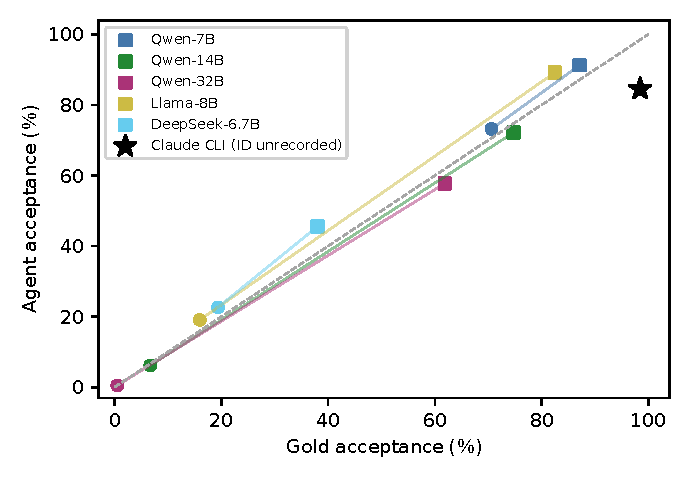
\includegraphics[width=0.82\linewidth]{generated/figures/dilemma_frontier.pdf}
\caption{Verified acceptance for five open reviewers under naive (circles) and adjusted
(squares) prompts. Their aggregate agent/gold rates correlate at $r=\dilemmaR$; this does
not establish an instance-level decision rule. The archived Claude CLI result (star;
snapshot unrecorded) has a larger gold--agent gap in this selected panel.}
\label{fig:frontier}
\end{figure}


\textbf{Archived failing-patch comparison.} Table~\ref{tab:ladder} retains the recorded
acceptance rates while exposing both denominators and the incorrect pass condition. For
example, Qwen-7B accepts $254/302$ failing candidates under that assertion, versus $169/194$
gold candidates on different tasks. This is a diagnostic reason to inspect instructions
and populations before interpreting acceptance. It is not an estimate of the causal effect
of test status. The hosted reviewer's $43/81$ rate likewise cannot establish that it alone
passes a clean negative control. Correctly informing the reviewer and comparing suitable
task populations would be needed to test that claim.

\begin{table}[t]
\centering
\caption{Archived adjusted reviews on different gold and failing task sets. Failing-patch
prompts incorrectly asserted test passage. These rates do not validate discrimination
under correct test information. $k/n$ denotes accepted/valid verdicts.}
\label{tab:ladder}
\footnotesize
\resizebox{\columnwidth}{!}{\begin{tabular}{lrrrr}
\toprule
Reviewer & Gold $k/n$ & Gold\% & Failing $k/n$ & Failing\% \\
\midrule
Qwen-7B & 169/194 & 87.1 & 254/302 & 84.1 \\
Qwen-14B & 145/194 & 74.7 & 200/302 & 66.2 \\
Qwen-32B & 120/194 & 61.9 & 120/302 & 39.7 \\
Llama-8B & 160/194 & 82.5 & 260/302 & 86.1 \\
DeepSeek-6.7B & 73/192 & 38.0 & 133/296 & 44.9 \\
Claude CLI & 191/194 & 98.5 & 43/81 & 53.1 \\
\bottomrule
\end{tabular}
}
\end{table}

\textbf{Hosted reviewer paired comparison.} On all $194$ Agentless Verified paired tasks,
the archived Claude CLI reviewer accepts $164/194$ agent and $191/194$ gold patches.
There are $29$ gold-only and $2$ agent-only accepted pairs (two-sided exact McNemar
$p\approx4.63\times10^{-7}$). The paired acceptance difference is
\frontGapPt{} points, with the archived bootstrap $95\%$ interval
$[\frontGapCIlo,\frontGapCIhi]$. This is a reviewer-specific statistical difference,
not demonstrated maintainer agreement or functional correctness. It coexists with high
gold acceptance in this sample, but the exact hosted snapshot is unrecorded and no
predeclared control threshold was applied. Pairwise agreement with open reviewers ranges
from approximately $-0.02$ to $0.13$; agreement with the pilot rater is
$\kappa=\frontKappaHuman$. These comparisons do not validate the reviewer as a maintainer
proxy, and we make no recommendation to use it for merge decisions.

\begin{figure}[t]
\centering
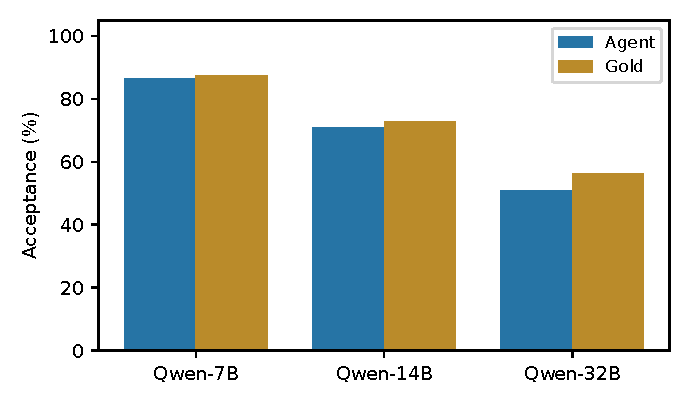
\includegraphics[width=\linewidth]{generated/figures/agent_vs_gold.pdf}
\caption{Adjusted Qwen acceptance rates on Lite. Agent and gold rates are close at each
reviewer size, while absolute acceptance varies by reviewer. Paired tests do not detect
differences here; non-significance is not equivalence.}
\label{fig:avg}
\end{figure}


Figure~\ref{fig:avg} shows the adjusted Qwen acceptance rates on Lite. Agent and gold rates
are close, while their absolute levels differ substantially by reviewer. Table~\ref{tab:dec}
reports the schema's decision categories: most non-merge actions are request-changes rather
than reject. A merge action can still fail the binary acceptance rule if it includes a
blocking issue, so action percentages need not equal RAP. The distribution alone does not
establish whether concerns are excessive or justified.

\begin{table}[t]
\centering
\caption{Decision distribution under the adjusted reviewers. Non-merge is dominated by
request-changes rather than reject, and agent and gold distributions track each other.}
\label{tab:dec}
\footnotesize
\begin{tabular}{lllrrr}
\toprule
Reviewer & Source & Split & Merge\% & Changes\% & Reject\% \\
\midrule
Qwen-7B & agent & Lite & 87.5 & 10.4 & 2.1 \\
Qwen-7B & gold & Lite & 89.6 & 9.4 & 1.0 \\
Qwen-7B & agent & Verified & 92.3 & 5.7 & 2.1 \\
Qwen-7B & gold & Verified & 88.7 & 7.7 & 3.6 \\
Qwen-14B & agent & Lite & 70.8 & 26.0 & 3.1 \\
Qwen-14B & gold & Lite & 72.9 & 24.0 & 3.1 \\
Qwen-14B & agent & Verified & 72.2 & 24.7 & 3.1 \\
Qwen-14B & gold & Verified & 74.7 & 22.2 & 3.1 \\
Qwen-32B & agent & Lite & 51.0 & 46.9 & 2.1 \\
Qwen-32B & gold & Lite & 56.2 & 42.7 & 1.0 \\
Qwen-32B & agent & Verified & 57.7 & 41.8 & 0.5 \\
Qwen-32B & gold & Verified & 61.9 & 37.6 & 0.5 \\
\bottomrule
\end{tabular}

\end{table}


\textbf{RQ3 (cited concerns).} We count reviewer-reported concerns without adjudicating
their truth. The naive prompt often cites insufficient tests (F7), consistent with the
omission of held-out tests from packets; the data do not identify that omission as the
sole cause. After the joint adjustment, F7 is rare in Qwen-14B's non-accepted agent verdicts
($1$ Lite patch, $0$ Verified patches). Regression risk (F2), fragility (F8), and convention
mismatch (F6) remain (Table~\ref{tab:tax}). Their factual validity and practical importance
require separate adjudication.

\begin{table}[t]
\centering
\caption{Failure modes cited on non-accepted agent patches under the adjusted
reviewer (count of patches flagged, any severity).}
\label{tab:tax}
\small
\begin{tabular}{llrr}
\toprule
Code & Cited concern & Lite & Verified \\
\midrule
F1 & Functional incompleteness & 9 & 7 \\
F2 & Regression risk & 6 & 18 \\
F4 & Non-minimal change & 5 & 11 \\
F5 & Maintainability & 3 & 8 \\
F6 & Convention mismatch & 11 & 11 \\
F7 & Insufficient tests & 1 & 0 \\
F8 & Fragile approach & 4 & 12 \\
F9 & API/compatibility & 1 & 3 \\
F10 & Performance & 1 & 2 \\
\bottomrule
\end{tabular}

\end{table}

\begin{table}[t]
\centering
\caption{Adjusted Qwen verdicts on gold. Gold blocking is the share reporting at least one blocking issue, not an adjudicated hallucination rate or the complement of gold acceptance.}
\label{tab:quality}
\footnotesize
\resizebox{\columnwidth}{!}{\begin{tabular}{llrrrr}
\toprule
Reviewer & Split & $n_g$ & Gold acc.\% & Gold blocking\% & Gold rej.\% \\
\midrule
Qwen-7B & Lite & 96 & 87.50 & 6.25 & 12.50 \\
Qwen-7B & Verified & 194 & 87.11 & 8.25 & 12.89 \\
Qwen-14B & Lite & 96 & 72.92 & 3.12 & 27.08 \\
Qwen-14B & Verified & 194 & 74.74 & 4.64 & 25.26 \\
Qwen-32B & Lite & 96 & 56.25 & 4.17 & 43.75 \\
Qwen-32B & Verified & 194 & 61.86 & 5.67 & 38.14 \\
\bottomrule
\end{tabular}
}
\end{table}


Table~\ref{tab:quality} distinguishes gold rejection from gold blocking. On Lite, Qwen-14B
rejects $26/96$ gold patches but reports blocking issues on only $3/96$. Across the adjusted
Qwen models and splits, gold blocking is $3$--$8\%$. A non-accepting decision can therefore
occur without a blocking label. These counts concern schema outputs, not whether the
underlying rationale is fabricated or a maintainer considered it.

\textbf{RQ4 (reviewer agreement).} Fleiss' $\kappa$ for the three adjusted Qwen models is
\fleissAllLite{} on all Lite packets and \fleissAllVerified{} on Verified. Adding Llama and
DeepSeek gives approximately $0.02$ on common valid Verified packets
(Table~\ref{tab:agree}). Thus model selection changes individual review decisions as well
as aggregate rates. A low $\kappa$ is chance-corrected disagreement in the tested panel;
it neither identifies which reviewer is correct nor validates the benchmark's historical
reference as an oracle.

\begin{table}[t]
\centering
\caption{Inter-reviewer agreement (Fleiss $\kappa$) on common valid packets. The five-reviewer panel includes Qwen, Llama, and DeepSeek; $a/g$ denote agent/gold.}
\label{tab:agree}
\small
\begin{tabular}{lrrrr}
\toprule
Panel / Split & $n$ packets & $\kappa_{all}$ & $\kappa_a$ & $\kappa_g$ \\
\midrule
Qwen / Lite & 192 & 0.1008 & 0.1327 & 0.0654 \\
Qwen / Verified & 388 & 0.1172 & 0.1222 & 0.1120 \\
Five / Verified & 383 & 0.0245 & 0.0471 & 0.0018 \\
\bottomrule
\end{tabular}

\end{table}





\textbf{RQ5 (coding-agent scaffolds).} We compare the adjusted Qwen panel on RAG+GPT-4
($14$ resolved tasks), SWE-agent+Claude-3.5 ($168$), Agentless+GPT-4o ($194$), and
OpenHands-CodeAct ($265$), each against gold on the same tasks (Table~\ref{tab:agents}).
The $2.8$--$53.0\%$ figures are official execution-based \%Resolved, not reviewer scores.
Qwen-14B does not detect a paired difference for any scaffold ($p=1.0$, $0.5601$,
$0.4996$, and $0.3891$). This statement must be reviewer-qualified: Qwen-32B accepts only
$35.1\%$ of SWE-agent patches versus $62.5\%$ of paired gold, and $29.8\%$ of OpenHands
patches versus $58.5\%$ of paired gold, with $p<0.001$ in both cases. The null does not
hold uniformly across the adjusted panel. Qwen-7B comparisons are non-significant, but
this does not establish equivalence. RAG's $14$ tasks and only two discordant pairs for
Qwen-14B provide little power, so we draw no evidence of equivalence from that result.
None of these tests establishes how maintainers would rank the scaffolds' patches.

\begin{table*}[t]
\centering
\caption{Across four agents spanning $2.8$--$53\%$ \%Resolved on Verified, adjusted Qwen results vary by reviewer. RAP is agent acceptance; each paired $p$ compares agent and gold on the same tasks. Qwen-32B detects differences for SWE-agent and OpenHands. RAG has low power.}
\label{tab:agents}
\small
\begin{tabular}{lrrrrrrrr}
\toprule
Coding agent & $n$ & \%Resolved & RAP$_7$ & RAP$_{14}$ & RAP$_{32}$ & $p_7$ & $p_{14}$ & $p_{32}$ \\
\midrule
RAG+GPT-4 & 14 & 2.8 & 92.9 & 78.6 & 50.0 & 1.0000 & 1.0000 & 0.2500 \\
SWE-agent+Claude-3.5 & 168 & 33.6 & 92.3 & 78.6 & 35.1 & 0.5235 & 0.5601 & $<0.001$ \\
Agentless+GPT-4o & 194 & 38.8 & 91.2 & 72.2 & 57.7 & 0.1516 & 0.4996 & 0.3497 \\
OpenHands-CodeAct & 265 & 53.0 & 89.4 & 79.2 & 29.8 & 0.7660 & 0.3891 & $<0.001$ \\
\bottomrule
\end{tabular}

\end{table*}


\subsection{Adapted binary-judge pilots}
\label{sec:adapted}
Following the preprints (Shi: arXiv:2511.10865v1), we adapt Cihan's classification task~\cite{cihanreview} and Shi's
\emph{unrefined draft-rubric ablation}~\cite{hitlpatch}, alongside a test-blind maintainer
comparator. All use the same pinned Qwen2.5-Coder-7B-Instruct, greedy decoding, full issue
and candidate diff, and binary JSON output; execution labels and candidate source are
hidden. Shi alone additionally derives a per-bug rubric from the developer patch.
Thus information access differs; this is not a reproduction of the full original systems.

Each pilot selects ten officially resolved and ten unresolved Agentless Verified tasks by
fixed hash order, subject to recorded length limits, and pairs agent/developer patches.
The first $120$ judgments produced $37$ Markdown-fenced JSON format failures under the
frozen strict parser; fence-only recovery is a separate post-hoc analysis. We then freeze
a fence-tolerant parser and a disjoint $20$-task follow-up before collecting its $120$
judgments (all valid), without changing judging prompts. Table~\ref{tab:adapted} reports
only this follow-up. Across both pilots there are $240$ judgments and $40$ rubric drafts.

\begin{table}[t]
\centering
\caption{Disjoint follow-up pilot: agreement with inherited functional labels on agent
patches (A), rejection of unresolved patches (N), and developer-patch acceptance (G).
These are adapted methods, not maintainer-validation or superiority results.}
\label{tab:adapted}
\footnotesize
\begin{tabular}{lrrr}
\toprule
Adapted judge & A ($n=20$) & N ($n=10$) & G ($n=20$) \\
\midrule
Maintainer & $14/20$ & $7/10$ & $9/20$ \\
Cihan & $13/20$ & $7/10$ & $8/20$ \\
Shi draft & $15/20$ & $6/10$ & $11/20$ \\
\bottomrule
\end{tabular}
\end{table}

Agreement's Wilson $95\%$ intervals are $48.1$--$85.5\%$, $43.3$--$81.9\%$, and
$53.1$--$88.8\%$, respectively. These small samples support no superiority claim.
Inherited execution labels are not new test runs or mergeability truth. Cihan's function
task is adapted to diffs without correction generation; Shi's two-human refinement and
human-consensus labels remain absent. Additional reference information also biases its
developer-patch acceptance. These pilots do not repair the archived negative inputs or
validate the historical reviewers.

A separately frozen extension evaluates all Lite ($300$) and Verified ($500$) gold
patches using the same test-blind maintainer adapter, without agent-based selection
or truncation. The $93$ shared tasks are evaluated once ($707$ unique gold), alongside
all $302$ available unresolved candidates; all $1,009$ calls complete, with three
malformed-JSON responses. Gold acceptance is $143/299$ valid on Lite and $284/499$
on Verified (one failure per split). Among $300$ valid same-task failing/developer
pairs, acceptance is $135/300$ versus $149/300$; discordant counts are $(47,61)$
(exact McNemar $p=.211$). Four empty candidates and two incomplete pairs are excluded
explicitly. This is not equivalence, new harness execution, or independent calibration.

\subsection{Qualitative inspection of cited concerns}
A post-hoc technical audit selects the first two nonaccepted hosted-reviewer cases in
lexical order within each of three strata: resolved agent ($30$ available), gold ($3$),
and failing agent ($38$). Archived diffs are applied to pinned upstream files; extracted
functions/branches run with synthetic inputs and backend stand-ins. Five focused claims
have local support; the gold \texttt{django-11179} regular-path stale-PK objection is
contradicted by existing cleanup. These checks are not independent adjudication or an
error-rate estimate. The \texttt{django-11555} phrase ``the one Django merged'' is a
recognition cue, not proof of training exposure.

For all three hosted nonaccepted gold cases, a separate $365$-day default-branch audit
finds $12$, $93$, and $35$ source-file commits (Django, Matplotlib, scikit-learn).
File churn is not defect count. Matplotlib issue \#27103 explicitly links the original
PR commit; fix \#27179 restores the default minimum to one and adds an empty-maximum
regression test, supporting the empty-bin concern. No matching regression was identified
for the other two concerns in this scoped inspection. This is not absence of defects;
other branches, renames and indirect effects are unmeasured. The public follow-up
predates the 2026 judging and may itself have been recognized.

\subsection{A human-review pilot}
Author Myeongmuk Kang, a non-independent, source-blinded rater, reviewed $40$ packets from
$20$ Agentless Verified paired tasks. The sampling script sorts task IDs, shuffles with \texttt{Random(7)}, selects
$20$, and then shuffles the $40$ agent/gold packets. The form uses the adjusted rubric,
but limits issues to $1{,}800$ characters and diffs to $9{,}000$, versus $6{,}000$ and
$24{,}000$ in the LLM path. Thus shared rubric does not mean identical input context.
The archive does not document Kang's prior code-review experience or precise role in rubric
development; these remain limitations rather than inferred credentials.

This rater accepts $15/20$ agent and $13/20$ gold packets ($75\%$ and $65\%$), with
paired $p=0.75$. Agreement with adjusted open reviewers ranges approximately from
$-0.22$ to $0.07$, and with the archived hosted reviewer is $\kappa=0.167$. This sample
provides descriptive observations only. It does not establish what humans in general would
accept, whether context truncation caused disagreement, or that any LLM or human escapes
an operational dilemma. Independent raters and context-controlled comparisons are needed
for such claims.

\section{Discussion}
\label{sec:discussion}
\subsection{Interpretation and diagnostic guidance}
\textbf{An acceptance rate needs a reference.} Gold outcomes offer a known historical
decision against which a reviewer can be compared cheaply, but not a defect-free truth
label. A worked example shows why the reference matters: on Lite the naive Qwen-14B
accepts $6/96$ agent patches and $5/96$ gold patches. The adjusted configuration accepts
$68/96$ and $70/96$, respectively. Reading only the agent column would suggest a large
change in patch quality even though the candidate patches are unchanged. The comparison
instead shows sensitivity to the assembled review configuration. It does not isolate
which prompt change caused that sensitivity. The diagnostic decision is to withhold
a mergeability interpretation for both configurations: historical-gold disagreement
limits the naive judge, while reused development tasks and the flawed failing-patch
condition leave the adjusted judge unvalidated. Higher acceptance alone is insufficient.

\textbf{Separate three questions.} Historical-gold agreement, sensitivity to functional
failure, and agreement with present-day maintainers are different outcomes. The paired
hosted result answers a reviewer-specific agent/gold question, and the pilot reports one
rater's judgments. The archived failing-patch rates answer neither functional-discrimination
under correct test information nor a causal test-status question. Consequently, neither
the hosted reviewer nor an open model is validated for real merge-decision support.

\textbf{A diagnostic protocol.} Future benchmark studies can (1) document source-blinded
packet contents and truthful test-status information, (2) report historical-gold acceptance
alongside agent acceptance, (3) develop rubrics using tasks separate from evaluation,
(4) introduce appropriate failing-patch controls with explicit task selection and accurate
instructions, (5) report valid counts, paired differences, missingness, and multiple-reviewer
agreement, and (6) obtain independent maintainer validation before making practical merge
recommendations. This is benchmark-design guidance, not a validated decision aid or a
universal numeric pass/fail rule. Our study demonstrates the need for these distinctions;
it does not claim to have completed every step.

\textbf{Scope of the observed tension.} The correlation across open configurations and
low agreement show dependence on judge choice in this sample. They do not identify a
single leniency mechanism or prove all open models incapable of discrimination.
Qwen-32B's cross-scaffold differences and the hosted operating point make a blanket
agent--gold null inaccurate. Model scale alone also does not explain the Qwen observations;
different checkpoints may have different training and alignment histories.

\textbf{Analysis reproduction versus fresh inference.} Stored labels and verdicts regenerate
tables and figures without model calls. New reviews require a serving environment; exact
hosted reproduction remains unresolved because its snapshot is unrecorded. Templates,
keys, verdicts, and regeneration code support computational checking, not adjudication or
recovery of missing identity.

\subsection{Threats to validity}
\textbf{Construct.} Historical merge outcomes can tolerate imperfections and depend on PR
discussion, CI, project plans, and social context absent from packets. Our binary labels
operationalize a reviewer decision, not a verified maintainer decision or an objection's
truth. The technical probes and three-case history audit provide no independent
rationale adjudication or population defect incidence. Historical merges can contain
defects. A single non-independent rater cannot supply that validation. Its shorter input limits further complicate human--LLM comparisons.

\textbf{Internal.} Rubric development reused the evaluation gold cohort, and intermediate
versions, inspected IDs, and iteration count were not preserved. Five subsets of fixed
verdicts do not establish task independence. The two prompt changes were not separated.
Negative-control inputs incorrectly asserted a pass and used disjoint task populations;
therefore their apparent separation cannot validate discrimination in the intended
condition. The hosted $81$-packet execution sample also has an unexplained missing position.

\textbf{Contamination and blinding.} Agents and reviewers may recognize public issues,
repository states or fixes. Explicit source masking cannot remove pretraining exposure;
either gold or agent acceptance could be affected, with unmeasured direction/magnitude.
Equal aggregate rates do not rule out recognition. This differs from documented gold-task
reuse in rubric development; public post-merge histories also predate the judging.

\textbf{External.} Selected Python tasks, four coding-agent prediction sets, five
open-weight reviewers and one unrecorded hosted snapshot do not cover all methods,
languages or model versions. Historical positive controls use resolved subsets;
the full-split extension covers only the test-blind 7B adapter. RAG's $14$ tasks support
no broad weak-agent claim. Industrial effort and deployment effects are unmeasured.

\textbf{Statistical and computational.} Tests are exploratory and use valid complete
pairs. Historical parsing, normalization and higher-temperature retries can affect the
population; their effects were not isolated. Wilson intervals rely on binomial assumptions;
aggregate correlations are descriptive. Non-significance is not equivalence, and low
agreement identifies no correct rater. Serving/numerical dependencies and the hosted
identity gap limit exact inference reproduction.

\section{Related Work}
\textbf{Execution and patch correctness.} Plausible but incorrect repairs are a longstanding
APR concern~\cite{overfitting,qirandom}. GenProg, Defects4J, and language-model
repair~\cite{legoues2012genprog,just2014defects4j,xia2022alpharepair,jiang2023impact}
motivate checking beyond available tests. Patch assessment uses behavioral or learned
evidence~\cite{patchcorrectness,patchsim}; our outcome is acceptance of repository review
packets relative to historical merge decisions.

\textbf{Human-guided assessment.} Shi et al.~\cite{hitlpatch} generate per-bug rubrics,
obtain human review/refinement, and judge patch validity against human consensus.
Cihan et al.~\cite{cihanreview} compare judgments of generated HumanEval code and
canonical solutions. Shared rubrics and positive controls are precedents, not our novelty.
Historical repository merges are not stronger truth than adjudicated human labels.
Our non-independent human pilot is not comparable validation; the additional method
adaptations in \S\ref{sec:adapted} likewise omit Shi's human-refinement stage.

\textbf{Review automation.} Industrial review includes design, conventions, and knowledge
transfer~\cite{modernreview,bacchelli2013review,rigby2013convergent}.
Tufano et al.~\cite{tufanoreview}, prompting/fine-tuning comparisons~\cite{promptreview},
LLaMA-Reviewer~\cite{llamareviewer}, and Atlassian's context-aware
RovoDev~\cite{rovodev} study review activities, comments, or revisions.
These objectives differ from our binary historical-acceptance comparison; we do not
reproduce all these systems or claim their deployment outcomes.

\textbf{Judge reliability.} LLM judges~\cite{llmjudge} exhibit comparison and self-preference
biases~\cite{wang2024fair,panickssery2024selfpref}. Our contribution is a SWE-bench-specific
diagnosis using historical gold, cross-agent paired decisions, and reviewer agreement,
with calibration reuse and flawed archived negative inputs explicitly limiting the claims.

\section{Conclusion}
Review-based scores require examining the judge as well as the patch. Historical prompt
adjustment changes agent and gold acceptance; reviewer/scaffold differences and paired
results do not establish equivalence or maintainer validity. The hosted identity is
missing and archived negative inputs are flawed. New full-split and matched controls
remain limited to a test-blind 7B adapter; targeted code/history checks establish no
population objection-error rate. Independent calibration and human validation remain
necessary before operational merge decisions.

\section*{Data and Artifact Availability}
Version \texttt{2026.11.05-v8} at
\url{https://github.com/myoungmuk/icse2027-6658-artifact-20261105-v2}
contains preserved inputs/outputs and regeneration instructions for historical analyses,
adapted pilots, full-split controls and technical/history checks. Analysis reproduction
does not recover the missing hosted identity or rubric history, or rerun inference.

\section*{Acknowledgments}
OpenAI Codex~\cite{openaicodex} assisted revision, analysis, figures, reference checks and
implementation. The authors are responsible for all claims and the final manuscript.

\clearpage
\bibliographystyle{IEEEtran}
\bibliography{references}

\end{document}
